\documentclass{article}
\usepackage{microtype}
\usepackage{graphicx}
\usepackage{subcaption}
\usepackage{booktabs}
\usepackage{hyperref}
\newcommand{\theHalgorithm}{\arabic{algorithm}}
\usepackage{icml2026}
\usepackage{amsmath,amssymb,mathtools}
\setlength{\bibsep}{0.5pt}

\newcommand{\selcand}{C0}
\newcommand{\selcandreason}{ -- no candidate passed hard validity; numbers below are reported for C0 descriptively}
\newcommand{\nstatestotal}{40}
\newcommand{\nstatespertask}{12/13/15}
\newcommand{\ncellstotal}{2,560}
\newcommand{\cellsps}{5.42}
\newcommand{\dwhA}{+0.041}
\newcommand{\dwhAlo}{+0.029}
\newcommand{\dwhAhi}{+0.053}
\newcommand{\dwhB}{-0.034}
\newcommand{\dwhBlo}{-0.073}
\newcommand{\dwhBhi}{+0.005}
\newcommand{\dwhC}{-0.130}
\newcommand{\dwhClo}{-0.161}
\newcommand{\dwhChi}{-0.100}
\newcommand{\resultsummary}{Applying the preregistered labeling rule descriptively, t1a straighten is labeled \emph{contact-dominant}; t1b single bend is labeled \emph{balanced/inconclusive}; t1c endpoint reposition is labeled \emph{direction-dominant} on this pilot.}
\newcommand{\crosscandsummary}{Across all 4 execution regimes (C0--C3), the sign of $\Delta_{WH}$ per task is \emph{not} consistent (Figure~\ref{fig:primary}); non-primary candidates are descriptive only.}
\newcommand{\interactionsummary}{Interaction estimates are t1a straighten: +0.228 [+0.217, +0.239]; t1b single bend: +0.154 [+0.138, +0.168]; t1c endpoint reposition: +0.007 [-0.007, +0.020]. The t1a and t1b estimates sit far above the zero-displacement noise floor; the t1c interval includes zero.}
\newcommand{\varsharesummary}{contact/motion/interaction variance as t1a straighten: 12\%/2\%/86\%; t1b single bend: 8\%/16\%/76\%; t1c endpoint reposition: 12\%/66\%/21\%.}
\newcommand{\vzerosummary}{t1a straighten: -0.151; t1b single bend: -0.142; t1c endpoint reposition: -0.066}
\newcommand{\hthree}{-0.180}
\newcommand{\hthreelo}{-0.201}
\newcommand{\hthreehi}{-0.160}
\newcommand{\hthreesummary}{The interval excludes zero.}
\newcommand{\guardplaceerrused}{$7.8{\times}10^{-5}$}
\newcommand{\guardnoopmed}{$1.0{\times}10^{-8}$}
\newcommand{\guardnooppninenine}{$9.1{\times}10^{-3}$}
\newcommand{\guardrepagree}{1.000}
\newcommand{\guardsettle}{0.9957}
\newcommand{\guardnonfinite}{0}
\newcommand{\guardinvrate}{0.2188}
\newcommand{\guardfactorgap}{$9.8{\times}10^{-3}$}
\newcommand{\zerodeltamed}{$1.4{\times}10^{-3}$}
\newcommand{\zerodeltapninenine}{$3.1{\times}10^{-3}$}
\newcommand{\guardlead}{The invalid-table rate guard fails: 42 of 192 tables are invalid (rate 0.219 $>$ 0.02), dominated by 6 states with a canonicalization re-placement artifact (error up to $6.4{\times}10^{-3}$); the registered 0.02 threshold admits less than one invalid table per candidate at this pilot scale, so under the strict fixed-priority rule no candidate regime is selectable. Invalid tables are quarantined, never averaged in, and listed in the released data. The full-state-set no-op p99 guard also fails, driven entirely by quarantined states; restricted to analyzed states, no-op drift is median $1.0{\times}10^{-8}$, p99 $1.5{\times}10^{-4}$, well within thresholds.}
\newcommand{\absguards}{Repeatability, drift, and noise-floor controls pass on all analyzed tables, but a canonicalization re-placement artifact invalidates 42/192 state tables (quarantined and reported separately) and makes the strict preregistered invalid-rate guard unsatisfiable at pilot scale, so no candidate regime is formally selectable and all numbers are descriptive.}
\newcommand{\primarytable}{\begin{tabular}{lcccc}
\toprule
Task & $n$ & $\Delta_{WH}$ & simult.\ 95\% CI & label \\
\midrule
t1a straighten & 12 & +0.041 & [+0.029, +0.053] & contact-dominant \\
t1b single bend & 13 & -0.034 & [-0.073, +0.005] & balanced/inconclusive \\
t1c endpoint reposition & 15 & -0.130 & [-0.161, -0.100] & direction-dominant \\
\bottomrule
\end{tabular}}
\newcommand{\decomptable}{\begin{tabular}{lccccc}
\toprule
Task & $v_0$ & $v_P{-}v_0$ & $v_U{-}v_0$ & $I$ & $v_{PU}{-}v_0$ \\
\midrule
t1a straighten & -0.151 & +0.078 & +0.037 & +0.228 & +0.343 \\
t1b single bend & -0.142 & +0.104 & +0.139 & +0.154 & +0.397 \\
t1c endpoint reposition & -0.066 & +0.083 & +0.214 & +0.007 & +0.304 \\
\bottomrule
\end{tabular}}


\icmltitlerunning{Diagnosing Contact and Direction in DLO Manipulation}

\begin{document}
\twocolumn[
\icmltitle{Where to Act or Which Way to Move?\\
Diagnosing Contact and Direction in\\
Deformable Object Manipulation}
\begin{icmlauthorlist}
  \icmlauthor{Anonymous Author}{anon}
\end{icmlauthorlist}
\icmlaffiliation{anon}{Anonymous Institution}
\icmlcorrespondingauthor{Anonymous Author}{anonymous@example.com}
\icmlkeywords{deformable object manipulation, factorial intervention, action attribution}
\vskip 0.3in
]
\printAffiliationsAndNotice{}

\begin{abstract}
Hybrid manipulation policies jointly choose a contact location $p$ and a
motion command $u$, so successful one-step behavior does not reveal whether
progress comes from choosing \emph{where} to act, which planar direction to
move, or their interaction. We introduce a preregistered complete-factorial
diagnostic for quasi-static deformable linear object (DLO) manipulation: for
each canonicalized rope state we execute all $8{\times}8$ combinations of
arc-length contact positions and fixed-magnitude planar motion directions and
compare the value of selecting contact alone, direction alone, and both. The
claim is parameterization-specific: we compare contact-location choice with
fixed-magnitude planar-direction choice, not ``where'' versus ``how'' in
general. On a development-split pilot of \nstatestotal{} valid C0 state tables
(\ncellstotal{} analyzed action cells) across three tasks, the descriptive
contrast $\Delta_{WH}=\mathbb{E}_s[v_P-v_U]$ is \dwhA~[\dwhAlo, \dwhAhi] for
straightening, \dwhB~[\dwhBlo, \dwhBhi] for single-bend shaping, and
\dwhC~[\dwhClo, \dwhChi] for endpoint repositioning (simultaneous 95\%
intervals). Applying the preregistered labeling rule descriptively yields
contact-dominant, balanced/inconclusive, and direction-dominant labels,
respectively. However, 42 of 192 state--candidate tables were invalid, mainly
due to a canonicalization re-placement artifact: no candidate execution
regime passed the preregistered invalid-table-rate guard, C0 (the
first-priority regime) was \emph{not} formally selected and is reported
descriptively, and no hidden-split confirmation or clean reproduction was
run. The contribution is a transparent, guard-audited action-attribution
protocol and pilot evidence, not confirmatory conclusions.
\end{abstract}

\section{Introduction}
Deformable linear objects (DLOs)---ropes, cables, wires---remain hard for
robots: state is high-dimensional and dynamics are contact-mediated and
underactuated~\citep{sanchez2018robotic,zhu2022challenges}. Practical systems
therefore act through \emph{hybrid} actions: a spatial choice of contact
location paired with a motion command, as in dense per-point critic and
affordance maps with a motion
head~\citep{zhou2023hacman,mo2021where2act,wu2023foresightful,
zeng2021transporter}. These architectures optimize the pair jointly and
benchmarks score only the joint outcome, so success does not reveal whether
it came from selecting \emph{where} to act (contact location), which planar
direction to move, or their pairing---yet that attribution decides whether
the next unit of modeling effort should buy denser contact maps, richer
motion generation, or joint reasoning.

We measure the attribution by direct intervention rather than by probing a
trained policy, in a deliberately small setting: one-step, quasi-static DLO
manipulation. For each canonicalized rope state we execute \emph{every}
cell of an $8{\times}8$ grid of contact positions $\times$ planar motion
directions in a GPU-parallel rod simulator~\citep{cao2026dlolab} and record
normalized one-step progress; the value of knowing \emph{where}, the
direction, or \emph{both} is then computable per state with no model in
between---classical factorial experimentation~\citep{montgomery2017design}
applied to an action space.

\paragraph{Narrow claim boundary.}
The two factors are \emph{not} symmetric in expressiveness: the contact
factor covers the rope's full normalized arc length at 8 points, while the
motion factor covers only 8 planar directions at a fixed displacement
magnitude---no magnitude, vertical, or rotational freedom. Equal
$8{\times}8$ cardinality equalizes search budget, not representational
completeness. All results therefore compare \emph{contact-location choice
versus fixed-magnitude planar-direction choice}, not ``where versus how'' in
general; observed dominance of either factor can partially reflect this
asymmetry.

\paragraph{Contributions.}
(i)~A preregistered~\citep{nosek2018preregistration} factorial design for
one-step DLO action attribution with explicit validity guards, a
complete-table-or-invalid policy separating invalid runs from valid null
results, and effect-blind fixed-priority candidate selection.
(ii)~A pilot execution on three tasks with complete raw tables, controls,
and cluster-bootstrap uncertainty, suggesting factor importance reverses
across tasks.
(iii)~An honest account of a qualification failure: a canonicalization
re-placement artifact invalidated 42 of 192 state--candidate tables and
tripped the invalid-table-rate guard, so no candidate regime was formally
selected; all numbers are descriptive development-split pilot evidence
(deviations in Section~\ref{sec:validity}).

\section{Related work}
\paragraph{DLO and deformable manipulation.}
DLOs are a canonical testbed for manipulation beyond rigid-body
assumptions~\citep{sanchez2018robotic,zhu2022challenges}. Prior work servos
object shape through estimated deformation
models~\citep{berenson2013manipulation,navarro2016automatic,yang2023modal},
learns rope dynamics or policies from
interaction~\citep{nair2017combining,wu2020learning,chi2022irp}, and
standardizes evaluation in simulation
benchmarks~\citep{lin2021softgym,cao2026dlolab}. We propose no new method;
we measure how much one-step progress each half of a hybrid action
carries---a quantity these evaluations do not report.

\paragraph{Dense contact affordances and spatial action selection.}
A prominent architectural family scores \emph{where} to act densely over
the object or scene: Where2Act~\citep{mo2021where2act},
DualAfford~\citep{zhao2023dualafford}, dense affordances for
deformables~\citep{wu2023foresightful}, HACMan's per-point critic
maps~\citep{zhou2023hacman}, and Transporter-style spatial action maps
for cables and fabrics~\citep{zeng2021transporter,seita2021learning}. These designs commit
capacity to the \emph{where} factor by construction; we ask when that
commitment is empirically justified for DLOs.

\paragraph{Hybrid and parameterized action selection.}
Discrete--continuous action spaces are formalized as parameterized-action
MDPs~\citep{masson2016reinforcement} with dedicated
architectures~\citep{hausknecht2016deep}; robotic instantiations couple a
discrete pick with continuous motion parameters,
e.g.\ TossingBot~\citep{zeng2020tossingbot}. This literature optimizes the
joint choice but does not quantify each factor's marginal value; our
factorial tables provide exactly that decomposition for one primitive.

\paragraph{Attribution and evaluation rigor.}
Our estimands are classical factorial
quantities~\citep{montgomery2017design} estimated with cluster
bootstrap~\citep{efron1993introduction}; the reporting responds to
reliability failures in empirical
RL~\citep{henderson2018deep,agarwal2021statistical} and preregistration
practice~\citep{nosek2018preregistration}.

\section{Study design}
\subsection{Environment, states, and primitive}
We use a GPU-parallel discrete-rod simulator built on a differentiable rod
solver~\citep{cao2026dlolab} with a 32-vertex rope. States are
\emph{canonicalized quasi-static} configurations: an analytic initial
centerline is placed, velocities are zeroed, and the rope is settled to a
velocity threshold of $10^{-3}$ (capped at $10^4$ steps). The primitive is
grasp--move--release--settle at a chosen vertex; grasp realism is disabled
so attachment is deterministic. Placement error after canonicalization is
guarded at $\le 10^{-4}$\,m per table (Section~\ref{sec:validity}).

Tasks are t1a \emph{straighten}, t1b \emph{single bend}, and t1c
\emph{endpoint reposition}, with stratified initial shapes (\{u\_bend,
s\_curve, random\_smooth\}; additionally \{straight\} for t1b/t1c). Task
error $D$ is a correspondence-$L_2$ distance to a goal template; a state is
eligible only if $D_{\text{before}} \ge 0.10$ (twice the success
threshold). Action quality is normalized one-step progress
$Y(p,u) = \bigl(D_{\text{before}} - D_{\text{after}}(p,u)\bigr)/
\max(D_{\text{before}}, 10^{-8})$, where $p$ is the contact location and
$u$ the motion direction: $Y=1$ solves the task in one step, $Y=0$ is no
progress, and $Y<0$ makes the state worse.

\subsection{Factorial grid, candidates, and experimental units}
\label{sec:units}
Contacts are 8 normalized arc-length positions $\sigma_i = i/7$ mapped to
the nearest native vertex; motions are 8 planar directions at $45^\circ$
increments. A \emph{candidate execution regime} fixes the primitive's
remaining free parameters---displacement magnitude and lift height---for an
entire run: C0 $(0.10\,\text{m}, \text{low})$, C1 $(0.05\,\text{m},
\text{low})$, C2 $(0.10\,\text{m}, \text{high})$, C3 $(0.05\,\text{m},
\text{high})$. Table~\ref{tab:units} gives the unit hierarchy and where
invalid tables are excluded. Candidate selection is \emph{fixed-priority
after hard validity}
(C0$\to$C1$\to$C2$\to$C3): the first candidate passing the hard validity
guards of Section~\ref{sec:validity} is selected; effect size, sign, and
$p$-values are never consulted. In this pilot \emph{no candidate passed}
(Section~\ref{sec:results}); C0, the preregistered first-priority
candidate, is reported descriptively.

\begin{table}[t]
\centering\small
\caption{Experimental-unit hierarchy: state $\to$ table $\to$ action cell,
replicated over candidates. Any cell failure or re-placement violation
invalidates the whole table (quarantined, never averaged in); analysis uses
only valid C0 tables.}
\label{tab:units}
\begin{tabular}{lr}
\toprule
Unit & Count \\
\midrule
Canonicalized states (16 per task) & 48 \\
Candidate execution regimes (C0--C3) & 4 \\
State--candidate tables ($48\times4$) & 192 \\
Action cells per table ($8\times8$) & 64 \\
Executed action cells & 12{,}288 \\
Invalid tables (C0/C1/C2/C3: 8/10/16/8) & 42 \\
Valid C0 tables analyzed (12/13/15 per task) & \nstatestotal{} \\
Analyzed action cells (\nstatestotal{}$\,\times 64$) & 2{,}560 \\
\bottomrule
\end{tabular}
\end{table}

\subsection{Estimands: reading an $8{\times}8$ table}
\label{sec:estimands}
Each complete table answers four increasingly informed queries: a uniformly
random cell earns the table mean in expectation; choosing only the
\emph{contact} well earns at best the best \emph{row} mean; choosing only
the \emph{direction} well at best the best \emph{column} mean; choosing
\emph{both}, the best cell. Per state: $v_0=\operatorname{mean}_{p,u} Y$;
$v_P=\max_p \operatorname{mean}_u Y$; $v_U=\max_u \operatorname{mean}_p Y$;
$v_{PU}=\max_{p,u} Y$.
The primary contrast per task is
$\Delta_{WH}=\mathbb{E}_s[v_P-v_U]$: positive means contact selection is
worth more than direction selection, negative the reverse. Secondary
estimands are the interaction $I=\mathbb{E}_s[v_{PU}-v_P-v_U+v_0]$ (joint
value neither marginal explains), oracle gain $\mathbb{E}_s[v_{PU}-v_0]$,
and two-way ANOVA variance shares. As maxima, $v_P$, $v_U$, $v_{PU}$ are
upward-biased under noise and $I$ inherits a positive bias; a
zero-displacement control (identical primitive, zero motion; $|Y|$ median
\zerodeltamed{}, p99 \zerodeltapninenine{}) sets the floor against which
we read $I$.

\subsection{Validity, statistics, and deviations}
\label{sec:validity}
A table is valid only if all 64 cells complete with successful grasp,
converged settle, finite outputs, and re-placement error of the
canonicalized state within the $10^{-4}$\,m reset guard; any failure
invalidates the whole table (one retry, no cell deletion, no post-hoc state
replacement). Invalid tables are reported separately from valid null
results. Guards cover no-op drift, repeatability (top-action equivalence,
tie tolerance $10^{-4}$), settle convergence, non-finite incidents,
invalid-table rate, and factor-dependent invalidity gaps.

Uncertainty uses a stratified (task $\times$ initial-shape) cluster
bootstrap over states with $10^4$ resamples~\citep{efron1993introduction};
the three per-task primary contrasts form one family with studentized
max-$t$ simultaneous 95\% intervals. The preregistered minimum absolute
effect is $0.02$; a task is labeled \emph{contact-dominant} only if
$\Delta_{WH}\ge 0.02$ with simultaneous lower bound $>0$,
\emph{direction-dominant} symmetrically, else
\emph{balanced/inconclusive}. Cross-task contrasts use the shared strata
\{u\_bend, s\_curve, random\_smooth\} with equal weights (a
composition-confound correction) and are exploratory.

\paragraph{Deviations from preregistration.}
(1)~\nstatespertask{} valid development-split states per task instead of
the registered 96/64; (2)~hidden-split confirmation and clean reproduction
were not executed; (3)~cross-task contrasts use the shared-strata
correction above; (4)~claim language is narrowed to contact-location versus
fixed-magnitude planar-direction choice; (5)~the registered
\emph{study-level} placement guard is operationalized per table: states
that cannot be re-placed within $10^{-4}$\,m yield invalid, quarantined
tables rather than aborting the study. Grid, candidates, priority order,
eligibility, guards, and estimands are unchanged.

\section{Results}
\label{sec:results}
\paragraph{Qualification.}
\textbf{No candidate execution regime passed the preregistered
invalid-table-rate guard; every number below is descriptive
development-split pilot evidence.} \guardlead{} The failure sits in the
execution substrate, not the hypothesis; quarantine kept the artifact out
of the estimates. Signal-level controls on the
analyzed tables pass: repeat
top-action equivalence \guardrepagree{} ($\ge 0.99$), settle convergence
\guardsettle{} ($\ge 0.95$), non-finite incidents \guardnonfinite{},
factor-dependent invalidity gap \guardfactorgap{}, placement error over
analyzed tables \guardplaceerrused{} ($\le 10^{-4}$). Throughput was
\cellsps{} valid action cells/s at 512 parallel environments.

\begin{table}[t]
\centering\small
\caption{Primary contrast $\Delta_{WH}=\mathbb{E}_s[v_P-v_U]$ per task
(candidate \selcand{}); studentized max-$t$ simultaneous 95\% CIs over the
three-task family; $n$ = valid states. Labels apply the preregistered rule
(minimum effect $0.02$) \emph{descriptively}; development split only.}
\label{tab:primary}
\resizebox{\columnwidth}{!}{\primarytable}
\end{table}

\begin{table}[t]
\centering\small
\caption{Factorial decomposition per task (candidate \selcand{}; state
means, pointwise 95\% bootstrap CIs). $I$ is upward-biased by noise;
compare with the zero-displacement floor (median \zerodeltamed, p99
\zerodeltapninenine).}
\label{tab:decomp}
\resizebox{\columnwidth}{!}{\decomptable}
\end{table}

\paragraph{Primary contrast: factor importance reverses across tasks.}
Table~\ref{tab:primary} and Figure~\ref{fig:primary} give $\Delta_{WH}$ per
task. \resultsummary{} Figure~\ref{fig:heatmaps} shows why: straightening
(t1a) tables vary far more across contact rows than direction
columns---once a good grasp point is chosen, many pull directions work;
endpoint repositioning (t1c) shows the reverse column striping.
\crosscandsummary{}

\paragraph{Decomposition and interaction.}
Table~\ref{tab:decomp} reports marginal and joint components.
\interactionsummary{} Variance shares of the mean tables attribute
\varsharesummary{} For t1a/t1b the interaction rivals or exceeds either main effect---the
best cell is a specific contact--direction \emph{pairing} neither marginal
predicts; for t1c it is negligible. On the shared strata, the exploratory t1c$-$t1a interaction difference
(preregistered as H3, recomputed under the shared-strata correction) is
\hthree{}~[\hthreelo, \hthreehi]. \hthreesummary{}

\begin{figure}[t]
\centering
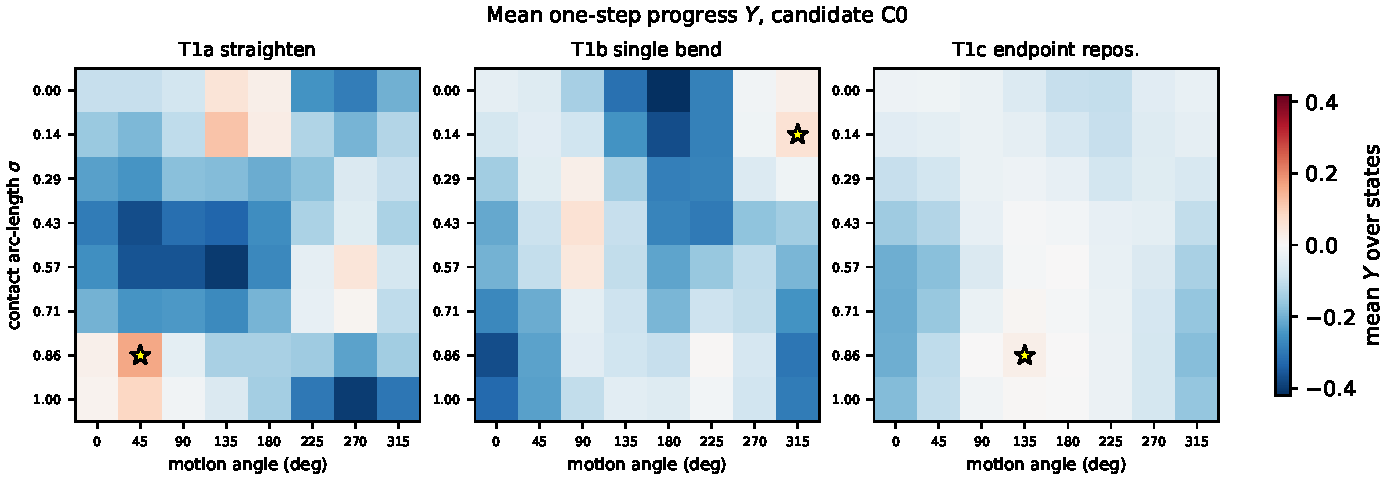
\includegraphics[width=0.96\linewidth]{fig_heatmaps.pdf}
\caption{Mean one-step progress $Y$ per task (candidate \selcand).
Rows: contact arc-length $\sigma$; columns: motion angle. Star: best mean
cell.}
\label{fig:heatmaps}
\end{figure}

\begin{figure}[t]
\centering
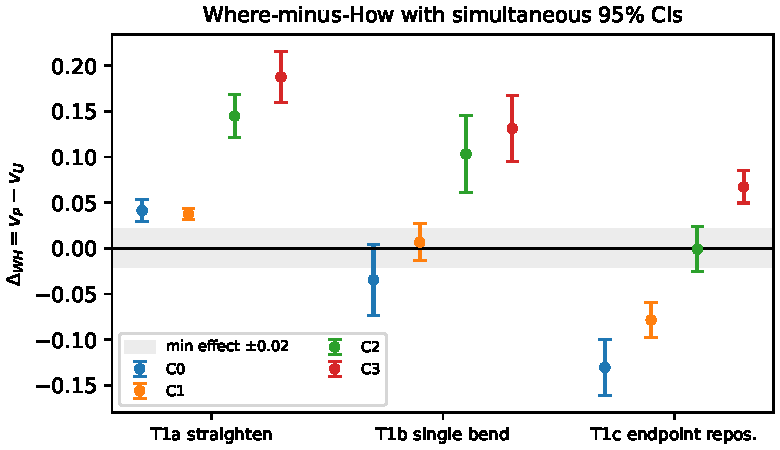
\includegraphics[width=0.84\linewidth]{fig_primary.pdf}
\caption{$\Delta_{WH}$ per task and candidate with simultaneous 95\%
intervals; shaded band is the preregistered minimum effect $\pm 0.02$.}
\label{fig:primary}
\end{figure}

\section{Discussion and limitations}
\paragraph{Interpreting direction dominance.}
A negative $\Delta_{WH}$ need not mean direction \emph{knowledge} is
constructively more valuable: a wrong direction actively harms ($Y<0$)
while a wrong contact is often merely unhelpful ($Y\approx 0$), so
direction dominance can reflect harm avoidance; the sign of $v_0$ (grand
mean \vzerosummary) bounds this share, and the expressiveness asymmetry of
Section~1 biases the same way.

\paragraph{Lessons for action parameterization design.}
First, \emph{equal cardinality does not equalize factors}: the contact
factor spans the rope's full arc length, the motion factor a thin slice of
motion space; attribution studies should publish such an expressiveness
audit (registered follow-ups: a $16{\times}16$ probe, a
magnitude-augmented motion factor). Second, \emph{factor
importance is a property of the task}: the sign of $\Delta_{WH}$ reverses
between straightening and endpoint repositioning. Architectures that
hard-code priority for one factor---dense where-maps with a coarse motion
head~\citep{mo2021where2act,wu2023foresightful,zhou2023hacman}---inherit a
task-dependent bias; sizable interactions on two of three tasks argue for
retaining joint contact--motion scoring.

\paragraph{Lessons for simulator benchmark design.}
(i)~\emph{Reset fidelity is a first-class property}: without per-table
placement checks the artifact would have silently biased every estimate;
simulators should expose and test deterministic
re-placement~\citep{lin2021softgym,cao2026dlolab}.
(ii)~\emph{Max-statistics need noise-floor controls}: best-of-table
quantities are upward-biased, so reported oracle or best-action gaps need a
sham control. (iii)~\emph{Guard thresholds must anticipate pilot scale}: a
0.02 invalid-rate threshold admits fewer than one invalid table per
candidate here, so one localized artifact makes the guard unsatisfiable;
thresholds should scale with sample size or carry explicit quarantine
semantics. We downgraded all claims rather than relax the threshold post
hoc; effect-blind selection makes the downgrade credible rather than
convenient~\citep{nosek2018preregistration,agarwal2021statistical}.

\paragraph{Limitations.}
This is a pilot: \nstatespertask{} states per task on the development
split, one simulator, one rope parameterization, no hidden-split
confirmation, no clean reproduction, no grasp realism. Effects are one-step
greedy quantities on canonicalized quasi-static states and do not license
multi-step policy conclusions; the motion factor omits magnitude, vertical,
and rotational components. Candidate-level evidence is unstable: the sign
of $\Delta_{WH}$ is not consistent across regimes
(Figure~\ref{fig:primary}), so labels are regime-specific. Wide intervals
mean \emph{balanced/inconclusive} reads as underpowered, not as evidence of
equality.

\section{Conclusion}
We contribute a preregistered, guard-audited pilot diagnostic attributing
one-step DLO progress to contact-location versus fixed-magnitude
planar-direction choice. Descriptively, contact choice mattered most for
straightening, direction choice for endpoint repositioning, with
substantial interactions on two of three tasks; because no candidate regime
passed the preregistered validity guard, these are pilot observations, not
confirmed findings. The design scales beyond the pilot; per-cell raw
data, configs, and seeds are released.

\clearpage
\bibliographystyle{icml2026}
\bibliography{references}

\end{document}
